%% start of file `template.tex'.
%% Copyright 2006-2013 Xavier Danaux (xdanaux@gmail.com).
%
% This work may be distributed and/or modified under the
% conditions of the LaTeX Project Public License version 1.3c,
% available at http://www.latex-project.org/lppl/.


\documentclass[11pt,a4paper,sans]{moderncv}        % possible options include font size ('10pt', '11pt' and '12pt'), paper size ('a4paper', 'letterpaper', 'a5paper', 'legalpaper', 'executivepaper' and 'landscape') and font family ('sans' and 'roman')

\usepackage[document]{ragged2e}
% pour justifier


% moderncv themes
\moderncvstyle{banking}                            % style options are 'casual' (default), 'classic', 'oldstyle' and 'banking'
\moderncvcolor{red}                                % color options 'blue' (default), 'orange', 'green', 'red', 'purple', 'grey' and 'black'
\renewcommand{\familydefault}{\rmdefault} 
%\nopagenumbers{} 
\usepackage[utf8]{inputenc} 
\usepackage[scale=0.9]{geometry}


\def \draft {1}
\usepackage{xparse}
\usepackage{ifthen}
\DeclareDocumentCommand{\comment}{o m o o o o}
{\ifthenelse{\draft=1}{
  \IfValueT{#1}{
      \textcolor{red}{\textbf{C (#1) : }#2}
      \IfValueT{#3}{\textcolor{blue}{\textbf{A1 : }#3}}
      \IfValueT{#4}{\textcolor{green}{\textbf{A2 : }#4}}
      \IfValueT{#5}{\textcolor{red!50!blue}{\textbf{A3 : }#5}}
      \IfValueT{#6}{\textcolor{blue}{\textbf{A4 : }#6}}
    }
    \IfNoValueT{#1}{
      \textcolor{red}{\textbf{C : }#2}
      \IfValueT{#3}{\textcolor{blue}{\textbf{A1 : }#3}}
      \IfValueT{#4}{\textcolor{green}{\textbf{A2 : }#4}}
      \IfValueT{#5}{\textcolor{red!50!blue}{\textbf{A3 : }#5}}
      \IfValueT{#6}{\textcolor{blue}{\textbf{A4 : }#6}}
    }
 }{}
}


\firstname{}
\lastname{}
\begin{document}

% recipient data
\recipient{Editor CEUS}{}
\date{\today}
\opening{Dear Editor,}
\closing{Yours faithfully,\\
Juste Raimbault and co-authors%\\
%Université Paris 7 - UMR CNRS 8504 Géographie-cités
}
         % use an optional argument to use a string other than "Enclosure", or redefine \enclname

\makelettertitle


%Dear Editor,

\justify


Thank you for the feedback on the draft paper ``Space Matters: extending sensitivity analysis to initial spatial conditions in geosimulation models''. The suggestions and comments will undoubtedly be of great value to the paper. It was updated accordingly.

\medskip

% Thank you for submitting your manuscript to Computers, Environment and Urban Systems. I have completed the review of your manuscript and a summary is appended below. The reviewers recommend reconsideration of your paper following major revision. I invite you to resubmit your manuscript after addressing all reviewer comments.

% When revising your paper, pay special attention to the explicit presentation of every model that is investigated in the paper. Present each model as an algorithm/unambiguous pseudocode and supply the Netlogo code for downloading (all this can be in appendix). The Schelling model, for example, has several Netlogo implementation, and it is critically important to know which of them is investigated. The same is true for the Sugarscape model. See comments of the reviewer #1 in this respect.

% When resubmitting your manuscript, please carefully consider all issues mentioned in the reviewers' comments, outline every change made point by point, and provide suitable rebuttals for any comments not addressed.




As a response to several reviewers, we made the following general changes:

\begin{itemize}
	\item Several comments, from the first and third referees especially, suggested that we clarify and explicit the description of our two models: we clarified the descriptions and justified our choices more thoroughly, and also provided pseudo-codes for each model in the Appendix so as to help the reader navigate the implementation chosen compared to other articles. Finally, we mentioned more clearly in the text the fact that source codes are openly available in a github repository.
    \item In order to conciliate as much as possible the different points of view about the comparison of phase diagram, we added some developments and comments about how we defined, built, justified and compared phase diagrams in the paper.
    \end{itemize}

\medskip



We now turn to point-by-point responses to referees comments.


\medskip


Concerning specifically the comments made by the first referee:

\begin{itemize}
	% 1. I think it would be better if the author would focus on a single model. This way they could describe the model and the analyses in more detail. As it stands, the models are treated as black boxes. 
	\item The suggestion to focus on a single model is a qualified comment. However, after presenting our research to several audiences, we came to the conclusion that the genericity of our approach would be better served by two case studies rather than with a single model. In that perspective, the ``black-box'' is seen as an advantage as it reinforces genericity. We acknowledge the fact that this choice led us to shorten the model presentations. Nevertheless, we have taken notice of your remark by improving the description of the models and their results through the addition of pseudo-codes in Appendix, result descriptions in the text and by recalling more clearly the link to the model source we used. Furthermore, we have focused on some of the most classical models of the ABM literature so as to lower the reader's cost of entry into the methodology.
   
   % I believe it would be better to begin with an illustrative example on how two or three initial patterns influence the model results and then use the suggested method for a more extensive analysis
   \item We agree that illustrative examples would provide a relevant starting point to  the analysis but we were afraid that their addition to the paper would make the introduction less straightforward and have the opposite effect to the one we were seeking. As we were nevertheless very interested by your remark, we provide a short answer to your proposition.
   
In order to get a first idea of the potential impact of spatial initial conditions on to the results of the simulation, we implemented on Segregation model a geographical constraint: some cells cannot be inhabited (yellow cells in Figure 1). The way those “forbidden” cells are distributed throughout space will indeed influence the steps of the model. 
We introduced various spatial initial conditions in the model that we controlled by one clustering parameter on the forbidden cells. A value of 0 would indicate a spatial distribution of yellow cells so as to minimize spatial autocorrelation. A value of 1 indicates on the contrary a concentration process that tends towards a high value of autocorrelation (see below Figure 1). % note : no fig envt in moderncv

We then compute the number of communities arising when the model converge, hence the number of different related components of similar neighbors.
Using 270 replications of 11 values of the clustering parameter (from 0 to 1 by step 0.1), we obtained a significant growth in terms of number of communities when the constraints on residential locations are concentrated in space, which might be interpreted in such example as a bigger segregation when density of housing is heterogeneously distributed through space. 
%In the rest of the article, we wish to further investigate such spatial effects in a much more systematic way.

%%%%%%%%%%%%%%
\begin{minipage}{\textwidth}
\begin{center} 
	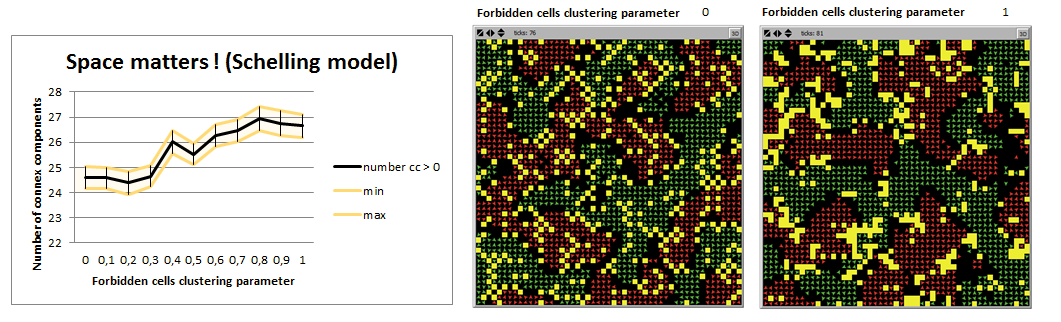
\includegraphics[width=\textwidth]{figures/SpaceMatters2.png}

\textbf{Effects of clustering of forbidden cells on the number of communities emerging from an adapted Schelling model (Netlogo implementation).}
\end{center}
\end{minipage}
%%%%%%%%%%%%%%
    
	% 2. It is very important to describe the models. This is especially relevant for the Schelling model, which has many variants; each has different dependencies on the initial pattern. In my opinion, the NetLogo implementation is not the best choice because the model does not reach a state of segregation when agents are highly intolerant.
	\item There was a misunderstanding for the Schelling implementation actually used, as we used our own implementation which pseudo-code has been added in Appendix of the paper and source code is openly available on the git repository of the project. This version implements the one used by (Gauvin et al., 2009), which also influenced us for the use of the term ``phase diagram''.

    \item More generally concerning the choice of these two models, we aim at helping the readers to distance themselves from the case studies and focus on the genericity of the approach. This also explains why we have chosen Sugarscape as a second example: these two models are often used as toy models due to the simplicity of their mechanisms and therefore do not require a high level of expertise nor technicality to apprehend the impacts of the initial spatial conditions on the model outputs. This is again an argument in favor of our choice: space-dependent variations are to be expected even with the most simple sociospatial models.
	
	% 3. I am not sure why the Sugarscape model has been chosen given that the paper seems to be focused on cities.
	\item Furthermore concerning the choice of the Sugarscape model, we think it is a good example of a stylized model of a spatialized socio-economic system, and according to (Batty, 2005) a good metaphor of an urban system. Our choice was accordingly clarified in the paper.
	
	% 4. Consider replacing “meta parameters” with something like “generator parameters” or “initial pattern parameters.”
	\item We agree that the term of meta-parameters may have been confusing, and following the suggestion we replaced it with ``generator parameters''.

	
	% 5. Line 228: Please explain why the median was chosen. Especially given that you use an L2 norm and variances in the index
    %\comment[JR]{je pensais qu'on prenait la moyenne ? je verifie... ligne 175 on écrit la médiane en effet}
	%\comment[CC]{ça doit être moi parce que je pensais qu'on prenait effectivement la médiane, qui est plus robuste aux extrêmes, mais si c'est la moyenne et que ça reste proche entre différentes réplications why not.}[(JR) il me semble que les distribs sont assez centrées et que ca revient quasiment au même ; par contre Clem si tu as pris median pour les stats et moi mean pour les plots c'est pas fou ; tu as encore le code des analyses stats ? (c'est sur le git ?)]
	%\comment[JR]{c'est la merde, on prend certaines fois la mediane et certaines fois la moyenne...}
    %\comment[FL]{certes c'est pas fou mais ca peut se défendre en disant que la médiane sert pour communiquer de façon accessible, sur une dimension pour laquelle c'était pertinent, mais que de façon générique on a préféré travailler sur la loi de Gauss car tout le monde à en tête ces indicateurs moyenne / ecartype c'est plus "passe partout"? }

	
	% 6. Line 232: comparing phase diagrams is related to the topic of comparing patterns. It would make sense to mention the methods that are usually used to compare patterns
	\item \comment[JR]{biblio a rajouter}
	
	% 7. Line 238: Please explain why this particular index was chosen and discuss its properties. Connect the discussion to other indices like L1, and Linf norms, etc. Would we get qualitatively different results from different indices? 
	\item The approach proposed in the paper is indeed rather exploratory. This explains why we have chosen to focus on a single index (L2) as this index is relatively well-known in the community. Previous exploratory analyses have shown that the results were rather stable when using the Monge method. Adapting the mathematical aggregator to the different indices would constitute an interesting perspective, but is out of the scope of the paper which already focuses on two models and proposes a new framework for analysing the impact of initial pattern parameters.
	
	% 8. Regarding the spatial generator: the authors should explain why this generator is relevant to these two models? 
	\item This spatial generator is relevant to both model as it produces density grids at a ``metropolitan scale'' (see detailed discussion added in Appendix and the original paper from which we used the generator), which is the scale at which both model were initially intended to be. We made this aspect more explicit. 
	
	\item In the case of Schelling, this is the scale at which most empirical segregation indices are computed. In the case of Sugarscape, it corresponds to the whole city if the model is a metaphor for city resources (Batty, 2005), or to a generic landscape where a resource is grown otherwise. In both cases, our point is that there exist many different patterns of density distribution in resource location and urban density, and that not acknowledging this diversity leads to potentially false results. Furthermore, in urban models, we argue that the hypothesis of isotropic density is potentially the most common simplification of the heterogeneity of space, with consequences on the model outputs often not evaluated.
	
	% 9. The authors should illustrate the contribution of each parameter of the generator to the generated initial pattern using a figure. Details of the generators should be included in an appendix
	\item The behavior of the spatial generator was described with more details in Appendix.
	
	% 10. Explain how the density grids are used in the Schelling model, do you allow more than one agent to be in the same cell? 
	\item Yes, we allow more agents to be in the same cell. The potential density is defined by the density grid generated, and its population with the same number of agents in all grids. This distribution is the one at initialisation. If the potential density is not reached, more agents can move in the cell, otherwise it is deemed full and unavailable for further moves. The satisfaction and segregation indices are computed with regard to the people in the cell and the people present in neighbouring cells.
	
	% 11. Line 297: I am not sure why empirical density destitutions of cities are important in the context of this study. 
	%\item cf infra. 
	\item Density distributions of empirical cities are important because we want to test models with realistic ranges of initial patterns of density distribution. Therefore we cannot limit ourselves to a single 2-peak mountain in the classical Sugarscape model and an isotropic square city in Schelling. We chose to use actual distribution of European cities to constraint our density generation.
	
	% 12. Line 641: NetLogo supports grids, continuous space, and GIS elements. It does not restrict the user in any way.
	\item We agree that NetLogo does not restrict the use on what implementation to use. However, some features are much more easier as raster or the contrary, which could influence the choice of beginners. Furthermore, models in the built-in NetLogo model library mostly rely on rasters. We clarified that statement in the paper.
	
	% 13. Line 301: I am not sure what the authors mean by “interesting grids”
	\item The term ``interesting grids'' was a typo and corrected, ``grids'' only was meant.
	
	% 14. Line 671: The same comment regarding “mythical ABMs” 
	\item The term ``mythical'' line 671 was a language mistake and corrected, ``textbook'' ABM was meant.
    %\comment[MLT]{Use "textbook ABM instead?}[(JR) yes, better]
\end{itemize}




Concerning the comments made by the second referee:

%This is an interesting article that I read with true interest. The paper fits the profile of this journal and can reach a wider audience.

%I also have some concerns:

\begin{itemize}
	% In the abstract the authors claim that initial spatial conditions are often taken for granted. I do not agree to this statement. Initial spatial condition can have a large impact on the results of a model, however I do not think that the initial spatial conditions are often taken for granted.
	\item We forcefully agree with the referee in that initial spatial conditions can have a large impact on the results of the model. Maybe not all papers take them for granted, but what we meant is that compared to other parameters, initial spatial conditions are much less often explored using sensitivity analysis. Actually, we know only a few papers which have explored the impact of initial spatial conditions as a systematic criterion in a sensitivity analysis of model results. We clarified this point in the introduction.

	% Page 2 line 88: the authors state that “Even in applied cases when GIS geometries of a particular city are used, the spatial distribution of agents is still approximated by a constant density”, I do not think this is true. Many models generate a heterogeneous synthetic population that is based on local data (replicating the actual population as closely as possible) and in far more detail then what is done in this paper. I am thinking of work in the line of disease diffusion, crime etc.
	\item We acknowledge the fact that many ABM applications use "real" data and spatial features for their simulations. However, as explained by (Thomas et al. 2017) in the case of LUTI models for instance, most simulations do not evaluate the impact of city delineations nor MAUP on the output of the models, which constitutes a potential limit in the interpretation of results.
	
	% Page 2 line 98: “However, this step is rarely explicit and authors tend to generalize the conclusion of the model from a single, spatial case study”. I do not understand the first part of the this statement. The steps taken are often very explicit. Due to the amount of time it takes to correctly represent all spatial data, including population densities and the variation of other population variables over space, many authors indeed restrict themselves to a single case study due to the time intensity of this task. Many agent-based models are also not valid for other areas.
	\item What we meant was actually that this step is rarely explicit and authors are therefore not able to generalize the conclusion of the simulations to other spatial context. We rephrased the paragraph accordingly.
	
	% The authors do not differentiate between data driven empirical models versus theory-driven models. I think a clear differentiation between the two groups and the positioning of the two case studies in the second group would make the paper more balanced.
	\item Concerning the remarks on synthetic population generation and the different types of models, we clearly stated our positioning regarding models built from theory, for which the proposed sensitivity analysis workflow is more suited and that our two case studies illustrate.
	
	% In section 1.3 (Previous considerations on the effects of the spatial configuration in simulation models) authors provide a lot of evidence on previous work on the impact of initial spatial conditions on the output of models. This is contrary to the statement in the abstract that initial conditions are often taken for granted.
	\item Indeed, we have tried to review articles where some kind of sensitivity to initial spatial conditions are tackled. However we would like to emphasize that the references cited in this section are few compared to the mass of geosimulation articles published with hardly any mention of dependence of output on initial spatial condition. Moreover, even if such sensitivity is analysed, it mostly provide some hints of impact of initial spatial conditions on the output of models (due to the accuracy of data, shape of boundaries and spatial heterogeneity) but to the best of our knowledge no article provide a systematic inquiry into the impact of systematically defined spatial input on the model output in the way we try to provide later on in the paper. We have tried to argue this point at the end of the section.
	
	% The most interesting part of the research to me, is not the way the density layers are generated but the use of the phase diagrams, defined as a vector of final aggregated model outputs. As these are vectors, they are not so different from time series and many techniques exist to compare vectors in this domain. I wonder if the Euclidean distance is the best measure to determine the difference between the phase vectors of different spatial inputs.
	\item The comment on other possible techniques to compare phase diagrams echoes one other reviewer comment, and we indeed expanded the discussion on this point, showing first that other distance do not change much qualitative results and with more literature for possible extensions.
	%\comment[JR]{analyse à ajouter}
	
	% Last paragraph of page 5, you do not state explicitly if genetic algorithms were use within the OpenMOLE platform.
	\item The functionalities of OpenMOLE we used were detailed in the article; we did not use genetic algorithms but sampling methods and high performance computing environments.
	
	% In section 3.1, page 8, line 404-405 the authors mention that the distance of the phase diagrams was measured with respect to the reference phase diagram computed on the default initial spatial conditions. Actually this came as a surprise to me. I had the impression that all phase diagrams would be evaluated against all other diagrams. Perhaps this should be explained earlier in the paper.
	\item \comment[JR]{ce qu'il suggère c'est un indice intégré sur l'ensemble des phases diagramme, donc un ``meta-meta-indice'' en quelque sorte, nous on reste à un niveau de meta seulement car on regarde juste pour chaque s'il bouge par rapport à un point de reference. En termes thematique c'est plus coherent pour nous, lui doit avoir en tete des indices de sensibilite globaux type Saltelli. $\rightarrow$ a voir comment justifier ca bien}{(JR) inclure en mise en contexte ce lien avec les Saltelli et indexes globaux}\comment[FL]{oui je trouve qu'on a le droit de rester limiter à cela c'est déjà pas mal!}
	
	% Figure 4 and 5: I find it confusing that the green color indicates higher distance values and the red color indicates lower values. I think this should be reversed.
    \item The double color progression in Fig 4 and 5 is used to highlight the opposition between ratio values above/under 1 but is not meant to introduce any hierarchy in the interpretation. We reversed the order of color according to your remark.
    %We would therefore prefer to keep the figures as they are if this is ok for you?
   	
	% I appreciate the fact that the authors in section 4 clearly indicate the limitations of their work (and I share the limitations listed under “comparing phase diagrams”). Personally I do not think that releasing the density grids is an important opportunity. As mentioned before I think that the core of the work is in the comparison of the phase vectors. I am not so sure the second opportunity listed in 4.2 is very valid. I do not think that the CEUS journal targets social sciences exactly.
	\item Thanks for the remarks on discussion, in particular on releasing density grids. We have tried to shorten the considerations which you have found not too useful and will let the readers decide if the grids could be of any use to them.
\end{itemize}





Concerning the comments made by the third referee:


\begin{itemize}
	% I found the research question posed by the author(s) interesting and I agree with the author(s) that many modelers don’t consider how spatial arrangements impact the outcomes of the model and tend to focus only on the parameters. The paper makes good use of the complexity and spatial literature in defining the problem and demonstrates how urban form impacts the results. However, while the paper is innovative, I found it really difficult to interpret and follow the results. I would suggest to the author to rewrite the results and methodology so that they flow better and also provide more context with respect to how to interpret the results.
	\item We have tried to make the methodology and result section flow better in the corresponding sections.
	
	% On a side note, one of your key words you use “validation” but in what sense?  You don’t really come back to this in the paper, also you write about “the validity of generative models is uncertain until their results are proven robust and representative of ’real-world’ conditions.” In the abstract but this is it.  What do you consider real world conditions to be? You seem to allude that you need to have the spatial generator to generate realistic (styles) city shapes for testing on the Schelling model but I am not convinced.  After the abstract all notion of validation is missing.
	\item We have agreed with the reviewer on ``validation'' and removed the concept of validation altogether, replacing it with model evaluation or sensitivity analysis.
	
	% Geosimulation is introduced but not defined or referenced.  This should be clarified as the term has several meanings etc.
	\item For the definition of geosimulation, we meant the one coined by (Benenson and Torrens, 2004), this was made explicit and the reference was added. 
    	
	% In places the English along with the overall argument could be better articulated. For example, on page 1 you write: “We think simulation can become a very good tool to achieve this,”  Could this be rewritten or better argued. You are not the only one to believe this but you don’t show this in your paper.
	\item We have worked towards improving the English along with the overall argument. 
	
	% Page 4: you write “Generally, sensitivity analyses have focused either on the spatial context (extent of the environment, shape of the zones if applicable - squares, hexagons, etc., objects - links, rasters, etc.); either on the spatial encoding of the heterogeneity of space (algorithms of disaggregation, interpolation, etc.), but rarely on both at the same time” This makes little sense. What it should be is “Generally, sensitivity analyses have focused either on the spatial context or the heterogeneity of space” or something like that. Basically you need the “or”.
	\item Thank you for the suggestion on page 4. We have modified the paragraph accordingly.


	% You write “To our knowledge there exist no single well established method to compare phase diagrams in the agent-based modelling and geosimulation literature.” As this is new you may want to discuss how say its done in other fields?  
	\item 
%    \comment[JR]{cf remarques other reviewers sur ce point}[(MLT) Sa remarque fait sens, mais j'avoue ne pas être trop au point sur cette partie de la littérature... vous avez des références?][(JR)concernant la spatial sensitivity : justement c'est pas trop fait non plus dans les autres champs ! je parlais avec un ecologue, leur espace est jamais varié autre que donnees reelles ; j'ai l'impressions que geosciences, hydrologie etc idem. Pour comparer phase diagrams j'ai pas en tete de domaine ou ca se ferait (faute d'avoir cherché, justement quand on cherchait une methode) - le plus proche c'est les patterns comparison etc. comme l'on suggere les reviewers.]
	
	% In the Schelling and sugarscape models how are the initial population of agents distributed? Is it random? I ask as this is unclear in the current version of the paper but it is vital if your purpose is to explore how the initial spatial configuration impacts the results of the model. Should the agents not be all located at the same location for each run to rule out the impact of initial placement of agents on the resulting patterns? This is something that is not addressed in the paper. I know for example, the Schelling model in NetLogo normally places the agents at random locations but in your reimplementation how is this done? The same goes for the sugarscape model in NetLogo. I believe a clearer description of the model initialization would be good and how its not the initial random placement of agents but the actual environment that impacts the outcomes. Maybe this was explained in the paper but I missed it.  
	\item Yes, classically, the initial distribution of agents is random in both models and, most importantly for our point, it follows a uniform distribution of density. In our implementation, the initial location of agents is also random in Schelling, but it follows a distribution of density given by the generated grid. In Sugarscape, the agents are initialised at random but the resources follow a distribution of density given by the generated grid. We have clarified this point in section 2.3
           
	% In Section 1.2 talk about “(monocentric vs. polycentric for example)” but in the results you don’t discuss the monocentric versions explicitly using these terms.
	\item We believe that the monocentric versions are explicitly analysed in table 1: the term "monocentric" itself does not appear in the regression results but it is only because it is taken as the reference case under the term "compact' in the regression. We have clarified this in section 3.2.
	
	% Also I appreciate you are trying to show rather complex results but reading the results several times I found the presentation of them (both written and visual) really hard to follow and understand. I was wondering if maybe you could find a better way to show / discuss them. Maybe a  worked example of how each set of parameters leads to a point in say Figure 4. Also it is confusing why the results from both models are not presented using the same styles of figures. For example, for the sugar scape model you different styles of figures than for the segregation model.
	\item Additional figures for the Schelling model presenting the results in a similar way were provided and commented in a way that tries to make it easier to grasp for the reader. Unfortunately, the figures showing grid estimates of phase diagrams could not be realized for the Schelling model because of the different sampling of the parameter space used.

\end{itemize}



 
Concerning the comments made by the fourth referee:


\begin{itemize}
	% In sensitivity analysis of spatial models, stochastic effects and small parameter changes are normally applied. What about initial conditions? The authors test the effects of different arrangements (e.g. monocentric vs. polycentric density patterns) on agent-based Schelling segregation models and Sugarscape's unequal societies model. Overall, I find this to be a very good paper. Very well written in general. Good review of the problem, clearly outlining (with references) the need for focus on initial conditions in geosimulation. The chief factors (data uncertainty, nature of spatial units (e.g. shape) and spatial heterogeneity) on initial spatial conditions are covered: -how many of these do you test? I see heterogeneity addressed, but what about shape and uncertainty? You touch upon shape when talking about NetLogo's use of raster as opposed to vector in the Discussion - could you expand on this?
	\item We thank the reviewer for this good remark. We provide references to papers addressing these issues. However, we have not addressed the shape of cells and the uncertainty of data in this paper, only the diversity of shapes of urban morphologies (e.g. heterogeneity). 
	
	% Rigorous experimental method described. In the matching of European metropolitan areas to your generated outputs, I wonder what you are missing by not using cities from other continents. i.e. by widening the cities available to your study it may be possible to even better discover real-world examples of your archtypes (compact, polycentric, discontinuous).
	\item To the best of our knowledge, there is no study of urban morphologies similar to the one we used but at a global scale (this should be linked to the absence of a raster of population with a resolution fine enough). Working on other regional systems of cities such as the US could be possible but remains out of the scope of this paper. We added this interesting suggestion to the discussion.
	
	% Why do you not have the same amount of repetitions for your Sugarscape (50 repetitions) and Schelling (100 repetitions) model runs?
	\item 
    %\comment[JR]{no justification for the difference in number of runs (just experimental setup contingence\ldots ) $\rightarrow$ either new runs or redo computations with 50 for Schelling}\comment[JR]{ca va etre chaud patate pour les new computations ; je vais regarder les ratio de sharpe, avec un peu de chance il y a besoin de plus de repets pour schelling...}
	
	% You say your models are open source - do you give details of that source?  
	\item Concerning the source code of the models, an open public repository was put into place and the link provided in the paper (to an anonymized version to ensure blind review). Similarly, the large simulation datasets used for results presented in the paper are openly available on a dataverse repository (provisorily anonymized also).
	%\comment[JR]{TODO dataverse. / statement open code and data}
	
	% Small edits:
	% X line 68: "...a different system"
	% figure 1: modify font size so that labels do not go to the edge of their respective objects
	% TODO Clem
	% figure 2: can you add the parameters that led to each of the grids
	% TODO Juste
	% figure 3: check spelling of "Augburg" (should be Augsburg)
	% TODO Clem
	% line 350: "...consists of..."
	% X line 455: "sa,e" = "same"? OK
	%figure 4 and figure 5 captions: make it explicit that we're seeing the Sugarscape results here.
	%line 515: "analyse" = "analysis"
	%line 593: "at reach" = "within reach"
	%line 671: would "classic" or "hypothetical" be better words (choice dependent on your meaning) than "mythical", which implies these are models of centuries ago and somehow out of reach..
	\item Spelling errors and approximations in the vocabulary chosen were corrected.
\end{itemize}







\justify




\makeletterclosing





\end{document}


%% end of file `template.tex'.